\documentclass[10pt, twocolumn, a4paper]{article}

\usepackage{graphicx}

\title{Hello, \LaTeX!}
\author{Mayank Bhagya}
\date{\today}

\begin{document}
\maketitle %this is important!

\begin{abstract}  
  This is a \textit{sample} document to \underline{experiment} with \textbf{LaTeX}.
\end{abstract}
  
\section{Introduction}

As shown in figure \ref{fig:satcount} on page \pageref{fig:satcount}, the number of active satellites have grown exponentially since 2016.

\begin{figure}[h]
  \centering
  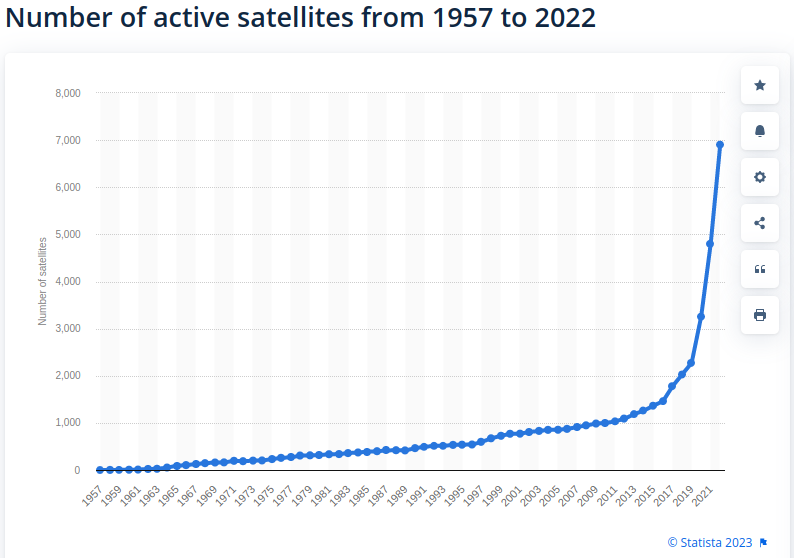
\includegraphics[width=\linewidth]{login}
  \caption{Active satellites by year}
  \label{fig:satcount}
\end{figure}

\section{Resources}

\subsection{Satellites}
Some of the most useful satellites for soil analysis are:
\begin{itemize}
  \item NASA Landsat
  \item ESA Sentinel
\end{itemize}

\subsection{Portals}
The data for these satellites can be obtained via the following portals:
\begin{enumerate}
  \item USGS
  \item Copernicus Open Access Hub
\end{enumerate}

\section{Misscelaneous}
The near infrared ($NIR$) and red ($R$) bands are used to compute vegetation index as per the equation:
\begin{equation}
  NDVI = \frac{NIR - R}{NIR + R}
\end{equation}

One last thing that remains is resolution and frequency of the satellites.
\begin{table}[h]
  \centering
  \begin{tabular}{|c|c|c|}
    \hline
    \textbf{Satellite} & \textbf{Spatial} & \textbf{Temporal} \\
    \hline
    Resourcesat & 30m & 6mo \\
    Landsat & 30m & 8d \\
    Sentinel & 10m & 5d \\
    \hline
  \end{tabular}
  \caption{Spatial and temporal resolutions of satellites.}
  \label{tab:resolutions}
\end{table}

We can also introduce greeks like $\alpha$, $\beta$, $\gamma$, $\delta$ or in large caps like $\Delta$. Also we can refer to any previous work that we've referred to \cite{overleaf} \cite{latextut}, while creating this doc by editing the *.bib file.

\bibliography{test}
\bibliographystyle{ieeetr}

\end{document}